\chapter{Background}

\label{Chapter2}

\lhead{Chapter 2. \emph{Background}}

%----------------------------------------------------------------------------------------
%	Initial Approach
%----------------------------------------------------------------------------------------

\section{Initial Approach}

\subsection{Assessing Project Scope}
The first problem encountered immediately in my project was in specifying
specifically what problem I wanted to solve, and which direction I should take
my project in. The initial proposition by my supervisor was very broad, 
enabling me to look into a wide variety of goals. In particular, I saw two separate areas
of focus -- there was a clear divide between looking \emph{within} individual git 
projects and comparing statistics \emph{between} multiple projects, with both 
enabling interesting data to be gathered. 

The possibilities of looking within projects is quite exciting, as it could enable a solution
to a problem that appears fairly regularly in industry -- the handover problem \cite{handover}.
For example, if we were to provide information about certain files and even lines which are 
often modified in commits, it could highlight an area with a high potential for error.
Further to this, we could integrate the git commit analyses with a testing
framework, creating a tool to indicate good and bad coders -- those who add
tests, those who frequently break them etc.

There is also interesting potential in examining the data given between different
git projects. When we consider undergraduate work in earlier years, there are a
large number of courseworks which have the same specification, completed by 
individuals. This will allow us to directly compare statistics on these pieces
of work and gain some insight into the students' workflow, and even how this
compares to their grade received. Some areas of note in this area include comparing
areas of code modified, their start and end times, and the methodologies used
by undergraduates vs. postgraduates working on the same projects. The results
could easily be cross referenced against their grades to indicate successful
or poor approaches.

\subsection{Code Similarity}
\label{CodeSimBegin}

I chose to look more closely at the problems surrounding the comparison of
multiple code repositories as this would open the door to building a tool which
could be of use to fellow students as they undertake programming exercises for
their studies. It's possible that a project in this area could also benefit lab
coordinators, aiding in marking and feedback. For example, following some of the
techniques mentioned above, an analysis of git habits could reveal important
correlations between grades and certain workflows which could aid feedback and teaching.

Taking the analysis further, I considered what other information we could gather
from multiple code bases. Given the students all work toward the same coursework
specification, and in many cases, even from the same skeleton files, it would be
interesting to see how their code itself is similar or different. In parsing
the students code and using a certain means to analyse it, there is a huge 
amount of analysis we could perform on the results. This would
deviate from the focus of version control, but could provide a wealth of 
information on the students' approach to exercises.

It is down this avenue that I felt investing my time would be most fruitful --
it would be very interesting to look into the similarities of student code,
possibly comparing the approach to the marks received. Students would be
able to look at this and see where they're particular approach differed
significantly from the top of the class' work (for example). We could also
highlight where a student came up with a particularly novel solution, if they
receive a high mark but with a low similarity to other pieces of work. This
would work well with a graphical representation of the code, as mocked up in
Figure \ref{fig:SimilarityVsGradeGraph}. Note the outlier, with a high grade but
low similarity, indicating a unique but good approach. It is also obvious how
this could be used to provide genericised feedback, for example ``everyone in
this cluster failed to spot the trick of calling function foo recursively''.

\begin{figure}[h!]
	\centering
		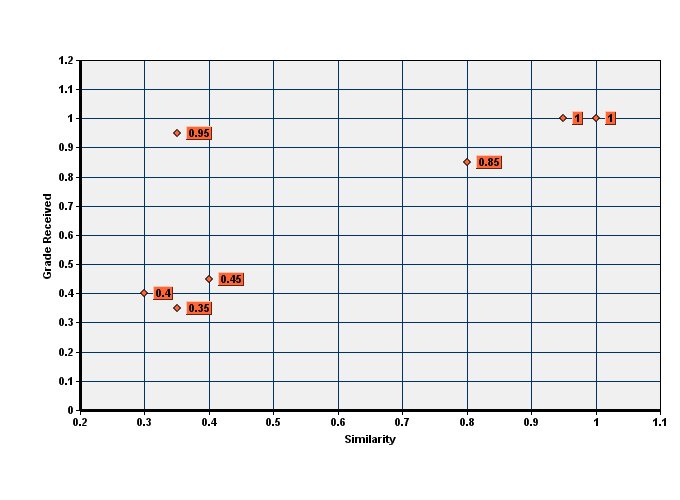
\includegraphics[width=\textwidth]{Figures/similarityVsGradeGraph}
	\caption{How a potential similarity graph may look, comparing each piece of
	code against the top graded work}
	\label{fig:SimilarityVsGradeGraph}
\end{figure}

I




%----------------------------------------------------------------------------------------
%	SECTION 2
%----------------------------------------------------------------------------------------

\section{Areas of Research}

Having discussed ideas with my proejct supervisor, and feeling happy with the
focus on code similarity, I proceeded to research academic articles which could
provide me with ideas and techniques to use in my project. We agreed that the
techniques used in plagiarism detection would be beneficial here, as what I aim
to achieve is essentially a less strict plagiarism detector. i.e. rather than
looking for a binary answer, ``yes'' vs. ``no'', to the similarity of code, I'd
want to find how similar the code is.

The issue of code similarity is a complex one, and solutions to the problem
vary wildly in terms of technique, complexity and accuracy. Although plagiarism
detection in essays and other extended writing tasks has been 
researched by many and a large number of working products exist, the research
into plagiarism detection within code is still a largely changing area. There
is currently no established norm to follow in building our solution. Our problem
is exacerbated by the fact that, as previously touched upon,
any research into plagiarism detection is
generally looking for a solution which can output a binary result, whereas the
aim of this project is to produce an output which gives a sliding scale.

My initial searches pointed me in the direction of the MOSS plagiarism detection
system. MOSS is a popular tool used throughout academia for detecting plagiarism
in code, which accepts a large number of input source code files and uses certain
techniques to check for plagiarism. The technique used is known as 
``winnowing''~\cite{winnowing}. This process takes ideas from earlier detection
techniques, such as \emph{k-grams}, and applies their own algorithms to indicate
code duplication. The winnowing algorithm works by hashing substrings of length
\emph{k} (the \emph{k-grams}) and moving through \emph{windows} of these hashes.
The winnowing step is the defined as: 
\begin{quote}In each window select the minimum hash value.
If there is more than one hash with the minimum value, select the rightmost
occurence. Now save all selected hashes as the fingerprints of the document.
\cite{winnowing}
\end{quote}

This process is undertaken after refactoring the code so that whitespace
has minimal effect and, if possible, variable renaming to normalised names.
The resulting fingerprints are then compared with the fingerprints of another
code base, with more hits indicating a larger likelihood of plagiarism.

We can see how this could be applicable for the uses of code similarity -- 
where code is written in a similar manner, more fingerprints would match,
giving us a clear similarity. Though this process works for plagiarism detection
where it is expected that code is simply lifted from one student's work to
another's, concerns can be raised as to how applicable this technique will work
when the code is similarly written, but not a direct copy. For example, when 
students are applying the same ideas to write their code, but not actually
copying each other, we would want to see a high similarity score. It is likely
that this may not result in a high score through winnowing due to constraints
with the algorithm. If the differences in layout happen to fall in an unfortunate
pattern, it's possible that the similarities are missed.

This technique does provide a possible solution to the issue of granularity of
similarity, as is discussed later in this chapter (section~\ref{subsec:SimGranularity}).

At the other end of the code comparison spectrum appears a detection framework
which examines the structure and semantics of code~\cite{Belkhouche}. This system
involves parsing the code and building an abstract syntax tree represenation.
From here, the tree is recursively divided into regions based on the control
flow of the program -- assignments are seen as leaf nodes, with comparisons being
subdivided further. See Figure~\ref{fig:BelkhoucheComparison} for an example of
the division into regions.

Once regions have been specified, we can now move on to the comparison steps,
which involve comparison of the \emph{syntactic catgeory} of the region, to 
remove unlikely matches in the code. For the remaining regions, the code
is then scrutinised more closely with a novel \emph{micro comparison} step -- 
looking at the shape and tokens of subtrees to look at similarity. The final step
compares the individual indentifiers in the subtree for similarity.

\begin{figure}[h]
	\centering
		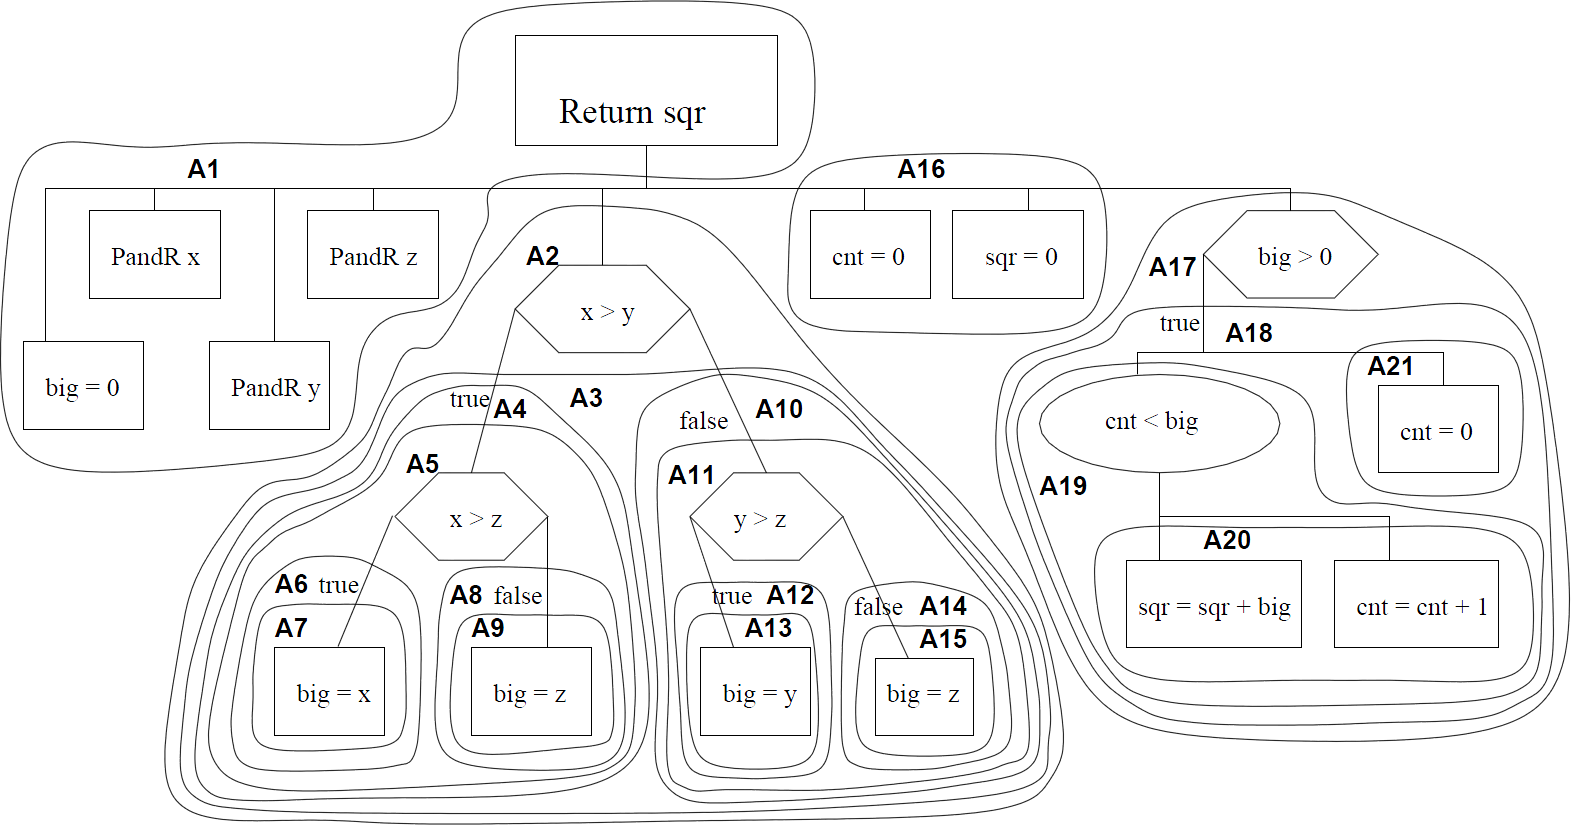
\includegraphics[width=\textwidth]{Figures/Belkhouche}
	\caption{Regions specified with Belkhouche et. al's method~\cite{Belkhouche}}
	\label{fig:BelkhoucheComparison}
\end{figure}

This technique has been proven to perform better than the previously discussed
winnowing algorithm for plagiarism detection. In this context, it is beneficial
as it is able to spot similarities that would otherwise go missed by winnowing.
This looks to be a good springboard for developing an algorithm to deal with
the issue of code similarity. Unfortunately,
the original research has since been destroyed, so a tool built upon this algorithm 
must be developed from scratch.

Further research into the semantic analysis to detect code similarities has yielded
a number of recent potential projects.



\section{Further Considerations}

There are some background tasks that also need to be researched further before a
well thought out plan can be finalised.

\subsection{Final Product Format}

A few options remain as to how the finished project should be presented to users.
Early ideas raised, before the projects direction was more firmly in place,
included Eclipse/IDE plugins or even an individual application. These are not a
viable approach to the problem as it is now described. Much more relevant formats
include building a web service which users could log in to, or even building a
gilab plugin. Currently, building a plugin for gitlab seems the most appropriate
solution to this issue. Students already have access to the gitlab internal website
and if there was an option to integrate these features with gitlab natively, it
seems the tool would be more straightforward, and therefore more useful, to use.

Having had minimal interaction with gitlab and it's source code in the past, this
approach, though very attractive currently, could be more problematic than 
initially thought. However, the software is open source, so it would be expected
that features such as this can be integrated with the local implementation
straightforwardly.

\subsection{Anonymising Code}

One of the key takeaways from this project is to give the students a tool
they can use to compare their code with their colleagues' code, in particular
looking at the grades received and thus what they can do to improve themselves.
However, this has implications on the privacy of their work -- it is simple to
anonymise the grades associated with the code by not including any names in
the comparisons. However, what is more difficult to hide is the circumstance where
students leave identifying information in their commit messages or code comments.

Depending on user feedback, different approaches can be implemented. The simplest
solution is to warn students that their code and commits will be viewable, so
they have the opportunity to remove any identifying information as they wish. It
could even be possible to allow students to opt-out of the system, removing them
from any data collected, but also forbidding them access to the system. A more
complex approach involves using already established algorithms to censor certain
information such as names and logins, though this may not be foolproof, and so
leaves the door open for unhappy students being identified.

\subsection{Data Representation}

Section~\ref{CodeSimBegin} presented a mockup of how the similarity scores could
be displayed in a graphical manner, however there are a multitude of ways that
this data could be presented. A main area of focus second to the algorithm should
be exactly how this information can be displayed -- the format should provide
clarity and ease of understanding, whilst also retaining as much of the information
as possible. This is an area that would be best explored once a working prototype
is in place, and different formats could be presented to testers allowing them
to provide vital UI feedback.

\subsection{Granularity of Simularity Comparison}
\label{subsec:SimGranularity}

Given that the outcomes of this tool is to provide information on/for undergraduate
computing students, we need to look at how our definition of similar code might
change depending on a few factors. If the students are working on their very first
Haskell exercise, we may find that the only way to get useful information out
of the comparison is if the code is examined in a very fine grained manner. When
the code is only four or five lines long, there is a much greater weight placed
on changing half a line of code than in a second year Operating Systems course.
The language used also needs to be taken into consideration for the same reason.
As such, a possible area of study is looking how to modify parameters supplied
to, and maybe developing heuristics for, the algorithm to specify how we want
to examine the code.

\subsection{Other Useful Comparisons}

There are also areas of note previously touched upon but not focussed to much on.
It would be nice to finish the project with a suite of tools to be used by either
the lab coordinators or the students themselves. This could involve information
on their commits, or perhaps integrating with testing environments to indicate
exactly how well the student is performing at a certain time/how they improved.